\documentclass[10pt,a4paper]{article}

% ---------- geometry ----------
\usepackage[left=1.5cm,right=1.5cm,top=2cm,bottom=1.2cm]{geometry}
\setlength{\parindent}{0pt}
\setlength{\parskip}{4pt plus 1pt}
\pagestyle{plain}

% ---------- fonts ----------
\usepackage[T1]{fontenc}
\usepackage[utf8]{inputenc}
\usepackage{lmodern}
\usepackage{microtype}

% ---------- math ----------
\usepackage{amsmath,amssymb,amsthm}

% ---------- graphics ----------
\usepackage{tikz}
\usetikzlibrary{arrows.meta,positioning,calc,backgrounds,fit,decorations.markings}
\usepackage{tcolorbox}
\tcbuselibrary{skins,breakable}
\usepackage{multicol}

% ---------- colors ----------
\usepackage{xcolor}
\definecolor{accent}{HTML}{059669}    % emerald-600
\definecolor{sky}{HTML}{0284C7}       % sky-600
\definecolor{rose}{HTML}{E11D48}      % rose-600
\definecolor{amber}{HTML}{D97706}     % amber-600
\definecolor{purple}{HTML}{7C3AED}    % violet-600
\definecolor{slate}{HTML}{475569}     % slate-600
\definecolor{lightbg}{HTML}{F0FDFA}   % teal-50
\definecolor{skybg}{HTML}{F0F9FF}     % sky-50
\definecolor{amberbg}{HTML}{FFFBEB}   % amber-50
\definecolor{rosebg}{HTML}{FFF1F2}    % rose-50
\definecolor{purplebg}{HTML}{F5F3FF}  % violet-50

% ---------- header ----------
\usepackage{fancyhdr}
\pagestyle{fancy}
\fancyhf{}
\renewcommand{\headrulewidth}{0.8pt}
\renewcommand{\headrule}{\hbox to\headwidth{\color{accent}\leaders\hrule height \headrulewidth\hfill}}
\lhead{\small\textbf{CS5800 -- Algorithms}}
\rhead{\small\textbf{Group Seminar Handout}}
\cfoot{\small\thepage}

% ---------- section style ----------
\usepackage{titlesec}
\titleformat{\section}{\Large\bfseries\color{accent}}{}{0em}{}[\vspace{-2pt}]
\titleformat{\subsection}{\large\bfseries\color{sky}}{}{0em}{}
\titleformat{\subsubsection}{\normalsize\bfseries\color{amber}}{}{0em}{}
\titlespacing*{\section}{0pt}{8pt}{3pt}
\titlespacing*{\subsection}{0pt}{6pt}{2pt}
\titlespacing*{\subsubsection}{0pt}{4pt}{1pt}

% ---------- tcolorbox styles ----------
\newtcolorbox{defbox}[1][]{%
  enhanced,colback=skybg,colframe=sky,
  coltitle=white,fonttitle=\bfseries,
  boxrule=0.8pt,arc=4pt,left=6pt,right=6pt,top=4pt,bottom=4pt,
  attach boxed title to top left={yshift=-2mm,xshift=4mm},
  boxed title style={colback=sky,arc=2pt,boxrule=0pt},
  title=#1}

\newtcolorbox{thmbox}[1][]{%
  enhanced,colback=amberbg,colframe=amber,
  coltitle=white,fonttitle=\bfseries,
  boxrule=0.8pt,arc=4pt,left=6pt,right=6pt,top=4pt,bottom=4pt,
  attach boxed title to top left={yshift=-2mm,xshift=4mm},
  boxed title style={colback=amber,arc=2pt,boxrule=0pt},
  title=#1}

\newtcolorbox{algbox}[1][]{%
  enhanced,colback=lightbg,colframe=accent,
  coltitle=white,fonttitle=\bfseries,
  boxrule=0.8pt,arc=4pt,left=6pt,right=6pt,top=4pt,bottom=4pt,
  attach boxed title to top left={yshift=-2mm,xshift=4mm},
  boxed title style={colback=accent,arc=2pt,boxrule=0pt},
  title=#1}

\newtcolorbox{notebox}{%
  enhanced,colback=purplebg,colframe=purple,
  boxrule=0.6pt,arc=3pt,left=6pt,right=6pt,top=3pt,bottom=3pt}

\newtcolorbox{resultbox}{%
  enhanced,colback=rosebg,colframe=rose,
  boxrule=0.8pt,arc=4pt,left=6pt,right=6pt,top=4pt,bottom=4pt}

% ---------- compact lists ----------
\usepackage{enumitem}
\setlist{nosep,leftmargin=14pt,itemsep=2pt}

% ---------- tikz styles ----------
\tikzset{
  fnode/.style={circle,draw=slate,fill=white,text=slate,
    minimum size=18pt,inner sep=0pt,font=\small\bfseries,line width=0.7pt},
  snode/.style={fnode,draw=sky,fill=sky!10,text=sky},
  tnode/.style={fnode,draw=rose,fill=rose!10,text=rose},
  fedge/.style={-{Stealth[length=4pt,width=3pt]},semithick,color=slate},
  pedge/.style={-{Stealth[length=4pt,width=3pt]},semithick,color=amber},
  bedge/.style={-{Stealth[length=3pt,width=2.5pt]},semithick,color=purple,dashed},
  cedge/.style={very thick,color=rose,dashed},
}

\newcommand{\cf}{c_f}
\newcommand{\Gf}{G_f}

\begin{document}

% ==================== TITLE ====================
\begin{center}
{\LARGE\bfseries\color{accent} The Ford-Fulkerson Algorithm}\\[3pt]
{\large\color{slate} Maximum Flow in Network Graphs}\\[2pt]
{\color{slate!60}\rule{0.4\textwidth}{0.4pt}}
\end{center}

% ==================== REAL WORLD MOTIVATION ====================
\section{Why Maximum Flow?}

Imagine a network of \textbf{drainage ditches} on a farm. Water flows from a pond through junctions to a creek, and each ditch has a limited capacity. \textit{What is the maximum amount of water we can drain per second?}

This is the \textbf{Maximum Flow Problem} --- it appears in network bandwidth, airline scheduling, bipartite matching, and more.

% ==================== FLOW NETWORK ====================
\section{Flow Network}

\begin{defbox}[Definition]
A \textbf{flow network} $G=(V,E)$ has a \textbf{source}~$s$, \textbf{sink}~$t$, and capacity $c(u,v)\geq 0$ on each edge.
A \textbf{flow}~$f$ assigns a value to each edge satisfying:

\begin{multicols}{2}
\begin{enumerate}
  \item \textbf{Capacity}: $0 \leq f(u,v) \leq c(u,v)$
  \item \textbf{Conservation}: $\displaystyle\sum_v f(v,u) = \sum_v f(u,v)$\; for $u\neq s,t$
\end{enumerate}
\end{multicols}
\vspace{-4pt}
The \textbf{flow value} is $|f| = \sum_v f(s,v) - \sum_v f(v,s)$ (net outflow from source).
\end{defbox}

\vspace{4pt}

\begin{center}
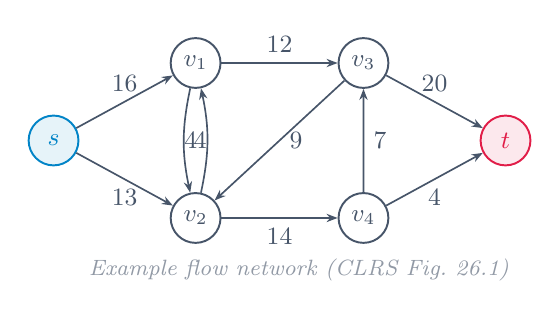
\begin{tikzpicture}[scale=0.82]
  \node[snode] (s)  at (0,0)    {$s$};
  \node[fnode] (v1) at (2.2,1.2)  {$v_1$};
  \node[fnode] (v2) at (2.2,-1.2) {$v_2$};
  \node[fnode] (v3) at (4.8,1.2)  {$v_3$};
  \node[fnode] (v4) at (4.8,-1.2) {$v_4$};
  \node[tnode] (t)  at (7,0)    {$t$};

  \draw[fedge] (s)  -- node[above,font=\small]{16} (v1);
  \draw[fedge] (s)  -- node[below,font=\small]{13} (v2);
  \draw[fedge] (v1) -- node[above,font=\small]{12} (v3);
  \draw[fedge] (v1) to[bend right=12] node[right,font=\small]{4}  (v2);
  \draw[fedge] (v2) to[bend right=12] node[left,font=\small]{4}   (v1);
  \draw[fedge] (v2) -- node[below,font=\small]{14} (v4);
  \draw[fedge] (v3) -- node[right,font=\small]{9}  (v2);
  \draw[fedge] (v3) -- node[above,font=\small]{20} (t);
  \draw[fedge] (v4) -- node[right,font=\small]{7}  (v3);
  \draw[fedge] (v4) -- node[below,font=\small]{4}  (t);

  \node[font=\footnotesize\itshape,color=slate!60] at (3.8,-2) {Example flow network (CLRS Fig.\ 26.1)};
\end{tikzpicture}
\end{center}

% ==================== RESIDUAL NETWORK ====================
\section{Residual Network \& Augmenting Paths}

\begin{minipage}[t]{0.52\textwidth}
\begin{defbox}[Residual Capacity]
Given flow $f$, the \textbf{residual capacity} of edge $(u,v)$:
\[
  \cf(u,v) = \begin{cases}
    c(u,v) - f(u,v) & \text{if } (u,v)\in E\\
    f(v,u)           & \text{if } (v,u)\in E\\
    0                & \text{otherwise}
  \end{cases}
\]
The \textbf{residual network} $\Gf = (V, E_f)$ with $E_f = \{(u,v) : \cf(u,v)>0\}$.
\end{defbox}
\end{minipage}\hfill
\begin{minipage}[t]{0.44\textwidth}
\begin{notebox}
\textbf{\color{purple}Why back-edges?}
\smallskip

Back-edges let the algorithm \textit{undo} earlier decisions. Without them, a greedy approach can get stuck at a sub-optimal flow. Back-edges are the key insight that makes Ford-Fulkerson \textit{optimal}.
\end{notebox}

\smallskip

An \textbf{augmenting path} is any $s \to t$ path in $\Gf$ with $\cf > 0$ on every edge. Its \textbf{bottleneck}: $\cf(p) = \min\{\cf(u,v) : (u,v) \in p\}$.
\end{minipage}

% ==================== ALGORITHM ====================
\section{The Ford-Fulkerson Method}

\begin{algbox}[Ford-Fulkerson Algorithm (with BFS)]
\begin{enumerate}
  \item \textbf{Initialize} all edge flows to zero: $f(u,v) = 0$ for all $(u,v) \in E$
  \item \textbf{While} there exists an augmenting path $p$ from $s$ to $t$ in $\Gf$:
  \begin{enumerate}[label=(\alph*)]
    \item Find $p$ using \textbf{BFS} on $\Gf$ (guarantees shortest path)
    \item Compute bottleneck: $\cf(p) = \min\{\cf(u,v) : (u,v) \in p\}$
    \item Update flow along $p$:
      \quad forward edge: $f(u,v) \mathrel{+}= \cf(p)$,
      \quad back-edge: $f(v,u) \mathrel{-}= \cf(p)$
  \end{enumerate}
  \item \textbf{Return} $f$ --- maximum flow reached!
\end{enumerate}
\vspace{2pt}
{\small\color{accent} Complexity: $O(VE^2)$ using BFS.}
\end{algbox}

\newpage

% ==================== PAGE 2: WORKED EXAMPLE ====================
\section{Step-by-Step Example}

Starting from the graph on page 1, all edge flows begin at $0$.

\begin{multicols}{2}

\subsubsection{Iteration 1\;\; \textcolor{amber}{$+12$}}

\textbf{BFS path}: $s \to v_1 \to v_3 \to t$\\
Bottleneck: $\min(16, 12, 20) = \mathbf{12}$

\begin{center}
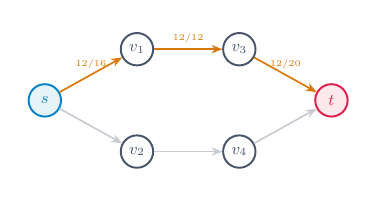
\begin{tikzpicture}[scale=0.65, every node/.style={transform shape}]
  \node[snode] (s) at (0,0){$s$}; \node[fnode] (v1) at (1.8,1){$v_1$};
  \node[fnode] (v2) at (1.8,-1){$v_2$}; \node[fnode] (v3) at (3.8,1){$v_3$};
  \node[fnode] (v4) at (3.8,-1){$v_4$}; \node[tnode] (t) at (5.6,0){$t$};
  \draw[pedge] (s)--node[above,font=\tiny]{\color{amber}12/16}(v1);
  \draw[pedge] (v1)--node[above,font=\tiny]{\color{amber}12/12}(v3);
  \draw[pedge] (v3)--node[above,font=\tiny]{\color{amber}12/20}(t);
  \draw[fedge,color=slate!30] (s)--(v2); \draw[fedge,color=slate!30] (v2)--(v4);
  \draw[fedge,color=slate!30] (v4)--(t);
\end{tikzpicture}
\end{center}
$|f| = 0 + 12 = \mathbf{12}$

\subsubsection{Iteration 2\;\; \textcolor{amber}{$+4$}}

\textbf{BFS path}: $s \to v_2 \to v_4 \to t$\\
Bottleneck: $\min(13, 14, 4) = \mathbf{4}$

\begin{center}
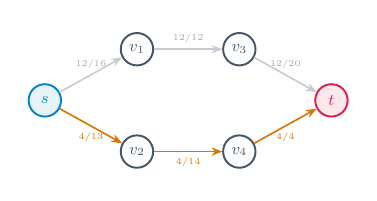
\begin{tikzpicture}[scale=0.65, every node/.style={transform shape}]
  \node[snode] (s) at (0,0){$s$}; \node[fnode] (v1) at (1.8,1){$v_1$};
  \node[fnode] (v2) at (1.8,-1){$v_2$}; \node[fnode] (v3) at (3.8,1){$v_3$};
  \node[fnode] (v4) at (3.8,-1){$v_4$}; \node[tnode] (t) at (5.6,0){$t$};
  \draw[fedge,color=slate!30] (s)--node[above,font=\tiny,color=slate!50]{12/16}(v1);
  \draw[pedge] (s)--node[below,font=\tiny]{\color{amber}4/13}(v2);
  \draw[fedge,color=slate!30] (v1)--node[above,font=\tiny,color=slate!50]{12/12}(v3);
  \draw[pedge] (v2)--node[below,font=\tiny]{\color{amber}4/14}(v4);
  \draw[fedge,color=slate!30] (v3)--node[above,font=\tiny,color=slate!50]{12/20}(t);
  \draw[pedge] (v4)--node[below,font=\tiny]{\color{amber}4/4}(t);
\end{tikzpicture}
\end{center}
$|f| = 12 + 4 = \mathbf{16}$

\columnbreak

\subsubsection{Iteration 3\;\; \textcolor{amber}{$+7$}}

\textbf{BFS path}: $s \to v_2 \to v_4 \to v_3 \to t$\\
Bottleneck: $\min(9, 10, 7, 8) = \mathbf{7}$

\begin{center}
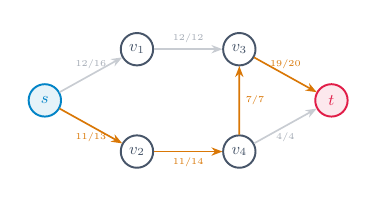
\begin{tikzpicture}[scale=0.65, every node/.style={transform shape}]
  \node[snode] (s) at (0,0){$s$}; \node[fnode] (v1) at (1.8,1){$v_1$};
  \node[fnode] (v2) at (1.8,-1){$v_2$}; \node[fnode] (v3) at (3.8,1){$v_3$};
  \node[fnode] (v4) at (3.8,-1){$v_4$}; \node[tnode] (t) at (5.6,0){$t$};
  \draw[fedge,color=slate!30] (s)--node[above,font=\tiny,color=slate!50]{12/16}(v1);
  \draw[pedge] (s)--node[below,font=\tiny]{\color{amber}11/13}(v2);
  \draw[fedge,color=slate!30] (v1)--node[above,font=\tiny,color=slate!50]{12/12}(v3);
  \draw[pedge] (v2)--node[below,font=\tiny]{\color{amber}11/14}(v4);
  \draw[pedge] (v4)--node[right,font=\tiny]{\color{amber}7/7}(v3);
  \draw[pedge] (v3)--node[above,font=\tiny]{\color{amber}19/20}(t);
  \draw[fedge,color=slate!30] (v4)--node[below,font=\tiny,color=slate!50]{4/4}(t);
\end{tikzpicture}
\end{center}
$|f| = 16 + 7 = \mathbf{23}$

\vspace{6pt}
\begin{resultbox}
\textbf{BFS finds no more augmenting paths.}\\[2pt]
After 3 iterations, maximum flow $|f^*| = \mathbf{23}$.
\end{resultbox}

\end{multicols}

% ==================== CUTS & THEOREM ====================
\section{Cuts and the Max-Flow Min-Cut Theorem}

\begin{minipage}[t]{0.52\textwidth}
\begin{defbox}[Definition: Cut]
A \textbf{cut} $(S,T)$ partitions vertices into $S \ni s$ and $T \ni t$.\\[2pt]
\textbf{Capacity}: $\displaystyle c(S,T) = \sum_{u\in S}\sum_{v\in T} c(u,v)$
\end{defbox}

\vspace{6pt}

\renewcommand{\arraystretch}{1.3}
{\small
\begin{tabular}{@{}llr@{}}
\textbf{\color{sky}Cut} & \textbf{$S$} & \textbf{$c(S,T)$}\\
\hline
Cut 1 & $\{s\}$ & $16+13 = \mathbf{29}$\\
Cut 2 & $\{s,v_1,v_2\}$ & $12+14 = \mathbf{26}$\\
\textcolor{rose}{\textbf{Min Cut}} & $\{s,v_1,v_2,v_4\}$ & $12+7+4 = \mathbf{\textcolor{rose}{23}}$\\
\end{tabular}}
\end{minipage}\hfill
\begin{minipage}[t]{0.44\textwidth}
\begin{center}
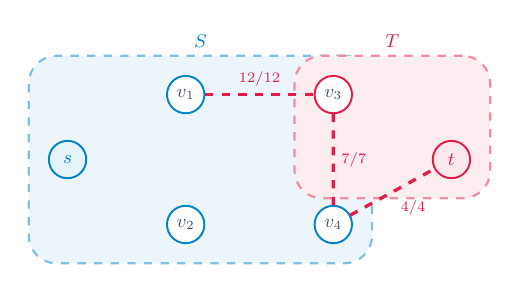
\begin{tikzpicture}[scale=0.75, every node/.style={transform shape}]
  \node[snode] (s) at (0,0){$s$};
  \node[fnode,draw=sky] (v1) at (2,1.1){$v_1$};
  \node[fnode,draw=sky] (v2) at (2,-1.1){$v_2$};
  \node[fnode,draw=rose] (v3) at (4.5,1.1){$v_3$};
  \node[fnode,draw=sky] (v4) at (4.5,-1.1){$v_4$};
  \node[tnode] (t) at (6.5,0){$t$};

  \begin{scope}[on background layer]
    \node[fit=(s)(v1)(v2)(v4),rounded corners=10pt,
          fill=sky!8,draw=sky!50,dashed,inner sep=7pt,line width=0.8pt] (sbox) {};
    \node[fit=(v3)(t),rounded corners=10pt,
          fill=rose!8,draw=rose!50,dashed,inner sep=7pt,line width=0.8pt] (tbox) {};
  \end{scope}
  \node[above,color=sky,font=\small\bfseries] at (sbox.north) {$S$};
  \node[above,color=rose,font=\small\bfseries] at (tbox.north) {$T$};

  \draw[cedge] (v1)--node[above,font=\scriptsize,color=rose]{12/12}(v3);
  \draw[cedge] (v4)--node[right,font=\scriptsize,color=rose]{7/7}(v3);
  \draw[cedge] (v4)--node[below right,font=\scriptsize,color=rose]{4/4}(t);
\end{tikzpicture}
\end{center}
\vspace{-2pt}
{\small\centering\itshape Min cut capacity: $12+7+4=23=|f^*|$\par}
\end{minipage}

\vspace{6pt}

\begin{thmbox}[Max-Flow Min-Cut Theorem]
The following three statements are \textbf{equivalent}:
\begin{enumerate}
  \item $f$ is a \textbf{maximum flow} in $G$
  \item The residual network $\Gf$ contains \textbf{no augmenting path}
  \item There exists a cut $(S,T)$ such that $|f| = c(S,T)$
\end{enumerate}
\end{thmbox}

\vspace{4pt}

\textbf{\color{accent}Proof sketch:}\;
When BFS fails to reach $t$ in $\Gf$, define $S=\{\text{nodes reachable from } s\}$ and $T=V\setminus S$.
Every $S{\to}T$ edge must be saturated (otherwise BFS would cross it), so $|f|=c(S,T)$.
Since $|f|\leq c(S',T')$ for \textit{any} cut, this flow is maximum and this cut is minimum.
\vspace{8pt}
\begin{center}
\colorbox{lightbg}{\parbox{0.9\textwidth}{\centering
\textbf{\large\color{accent} Key Takeaways}\\[4pt]
\begin{minipage}{0.9\textwidth}
\begin{enumerate}
  \item \textbf{\color{sky}Residual Network} $\Gf$ shows remaining capacity + back-edges for undo
  \item \textbf{\color{amber}Augmenting Path}: $s{\to}t$ path in $\Gf$; use \textbf{BFS} for $O(VE^2)$ guarantee
  \item \textbf{\color{rose}Max-Flow = Min-Cut}: algorithm stops when no path exists; flow equals min cut
\end{enumerate}
\end{minipage}}}
\end{center}

\end{document}
